% !TeX spellcheck = en_US
%Publications.tex
%\newcommand{\PublicationsPath}{PatentsAndPublications/Publications}

%MTAP2020

\section[Multi-access Edge Computing video analytics of ITU-T P.1203 Quality of Experience for streaming monitoring in dense client cells]{Multi-access Edge Computing video analytics of ITU-T P.1203 Quality of Experience for streaming monitoring in dense client cells}
\label{chap:MTAP2020}
\begin{itemize} \itemsep1pt\parskip0pt\parsep0pt
	\item \textbf{Title:} Multi-access Edge Computing video analytics of ITU-T P.1203 Quality of Experience for streaming monitoring in dense client cells
	\item \textbf{Authors:} Roberto Viola, Mikel Zorrilla, Pablo Angueira and Jon Montalb\'an
	\item \textbf{Journal:} Multimedia Tools and Applications
	\item \textbf{Publisher:} Springer
	\item \textbf{Year:} (Submitted March 25, 2021)
%	\item \textbf{DOI:}  \url{}
\end{itemize}	

\textbf{Abstract:} 5G promises unseen network rates and capacity. Furthermore, 5G ambitions agile networking for specific service traffic catalysing the application and network symbiosis. Nowadays, the video streaming services consume lots of networking assets and produce high dynamics caused by players mobility meaning a challenging traffic for network management. The Quality of Experience (QoE) metric defined by \hbox{ITU-T P.1203} formulates the playback issues related to widely employed Dynamic Adaptive Streaming over HTTP (DASH) technologies based on a set of parameters measured at the video player. Monitoring the individual QoE is essential to dynamically provide the best experience to each user in a cell, while video players compete to enhance their individual QoE and cause high network performance dynamics. The edge systems have a perfect position to bring live coordination to dense and dynamic environments, but they are not aware of QoE experienced by each video player. This work proposes a mechanism to assess QoE scores from network dynamics at the cell and manifests of DASH streams without an explicit out of band messaging from video players to edge systems. Hence, this paper implements an edge proxy, independent from video servers and players, to monitor and estimate QoE providing the required information to later decide streaming qualities in a coordinated manner in a dense client cell. Its lightweight computation design provides real-time and distributed processing of local sessions. To check its validity, a WiFi setup has been exercised where the accuracy of the system at the edge is checked by assessing the ITU-T P.1203 QoE of individual players.

\textbf{Keywords:} 5G, MEC, MOS, MPEG-DASH, QoE.

\subsection{Introduction}
\label{intro}

Popularity of video streaming platforms to consume live sports events and over-the-top (OTT) services like Netflix, when combined with mobility and city contexts, result in a complex traffic congestion scenario to be managed. Specifically, when video players share the same path, they try to individually enhance their Quality of Experience (QoE) considering instant available bandwidth and display setup. As the cell gets more subscribers and the Base Station (BS) serves more traffic sessions, dynamics turn higher and available bandwidth estimation at client side gets coarser, fuelling video player fluctuations on requested bandwidth which affect the QoE \cite{khan2018}. Therefore, when congestion at the radio link comes into place, a dense client cell means a pool of clients competing for the available network assets. This competition leads to player instability, unfairness between players, and bandwidth under-utilization \cite{akhshabi2012}.

Maximizing customer satisfaction through QoE-based networking is a crucial challenge for video streaming services.
As most of the traffic flooding the networks comes from video streaming services, Mobile Network Operators (MNOs) need to configure the network according to cost-effective policies to cope with video demand while providing best QoE with the available resources.
To this end, MNOs need to monitor the QoE without access to video streaming servers, Content Delivery Network (CDN) systems or video player applications.

In the upcoming horizon 5G aims to improve current Key Performance Indicators (KPIs), such as traffic density, volume and latency. It will flatten barriers to allow network operators and/or 3rd parties to provide dynamic networking performance to respond to specific traffic demands \cite{etsits5g}.
To this end, network management frameworks analyse network assets and traffic features to adapt network setup to concurrent traffic needs. This means a revolution on networks with a digital transformation which leaves behind the concept one-fits-all and moves to a specialized and mutable network which dynamically changes its configuration over a common bare-metal infrastructure.

In the line of catalysing synergies of network and traffic from services, edge computing is gaining relevance due to benefits of local processing. Enabled by the transition of networking assets to cloud infrastructures, the provision of hosting at the edge means new revenues for MNOs. Furthermore, the location of some parts or entire systems of a service closed to the clients enables advanced possibilities considering the user environment. The application of analytics at the edge to optimise the video streaming traffic is a use case compiled in the ETSI working documents as a key representative of Multi-access Edge Computing (MEC) application \cite{etsigsmec002}.

The proposed 5G MEC-enabled proxy estimates the end users' QoE according to ITU-T P.1203 \cite{itup1203} and derived from monitored QoS metrics in the radio cell to allow a decision by other edge services operating streaming qualities in a coordinated manner in a dense client cell. Thus, the proposed system catalyses the use of Video Streaming Analytics at the network edge to realise the network/application symbiosis \cite{etsigsmec002}.

The major contributions of this paper can be summarized as follows:
\begin{itemize}
	\item A novel mechanism to estimate ITU-T P.1203 \cite{itup1203} QoE values from network dynamics at the cell and parameters parsed from manifests of DASH streams without an explicit out of band messaging from video players to edge system.
	\item A lightweight implementation of an edge computing proxy, independent from video servers and players, to monitor and assess in real-time ITU-T P.1203 QoE values for each local session.
	\item The analysis of the accuracy of the proposed system to assess the ITU-T P.1203 QoE of individual players in a WiFi-based experimentation setup and a dense client cell. To this end, two scenarios with different levels of concurrency and congestion are performed.
\end{itemize}

The rest of this paper is organized as follows. First, the related work is in Section \ref{sec:MTAP20202}. The MEC system model and architecture and the streaming analytics service is in Section \ref{sec:MTAP20203}.
Furthermore, the system performance analysis, defined metrics, the evaluation setup and the results are described in Section \ref{sec:MTAP20204}. Finally, the Section \ref{sec:MTAP20205} concludes the paper.

\subsection{Related Work}
\label{sec:MTAP20202}

QoE of streamed video contents is intrinsically related to customers' satisfaction. Mean Opinion Score (MOS) compiles the results of subjective evaluations over a variety of representative spectators/audience surveyed to score perceived quality, ranging 1 to 5 values \cite{Itu2016}. However, this surveys process results in high expensive costs since it cannot be automated, as it is difficult to be repeated as updates on operational parameters are applied and it is complex to process the results in real-time.

Therefore, research community investigates models to map subjective distortion to objective QoS and application metrics which can be automatically monitored and computed in real-time producing actionable data \cite{Juluri2015}.
These subjective quality models change as the streaming technologies evolves. Nowadays, HTTP Adaptive Streaming (HAS) technologies are widely used for live and \hbox{on-demand} video streaming services. Then, QoE models shift from \hbox{pixel-level} distance evaluation of received frames from the original served, such as Peak Signal to Noise Ratio (PSNR) based on Mean Squared Error (MSE) or Structural Similarity Index (SSIM), to \hbox{content-agnostic} models with sophisticated parametric equations comprising throughput, frequency of bitrate changes from available representations and buffering duration. These models better reflect quality level from a video streaming perspective, they are lightweight and can be processed in \hbox{real-time}. \hbox{Per-title} encoding techniques \cite{cock2016} are widely employed by major video services, adapting the employed bitrate to the image complexity to save bandwidth costs, so representation bitrate has a direct translation to image fidelity and \hbox{pixel-level} distortion is not required anymore.

Objective QoE models \cite{liotou2016} are widely employed at media player side to enable decision making on representation/bitrate selection to accommodate the demand to the available network resources and maximise the local QoE. Some of the QoE models at player side are heavily dependent on buffer metrics \cite{huang2018}. At the server side, buffer information is not available and QoE models usually employ HTTP delivery information \cite{mangla2017}. Some server-side models exploit also lower-level information, such as TCP connections \cite{mangla2018}, or combine both TCP and HTTP information \cite{mazhar2018}. The ITU-T P.1203, whose last version was published in October 2017, is a standardized model for QoE evaluation of adaptive audio and video streams including video and audio quality and buffering issues, where quality is closely related to representation bitrate of each played media segment, number of representation switches, number of stalling events and their duration.

Dense client cells are tough environments where the autonomous decisions from video players may produce unfair, biased, unsteady and inefficient use of the radio link. There, intrinsic ON-OFF periods of HAS technologies may cause oscillations on the experienced network throughput and, accordingly, on the selected bitrate \cite{akhshabi2012}. Client-side algorithms, selecting representation to be downloaded and played, have been proposed to detect and compensate bitrate oscillations \cite{mueller2015}. However, the lack of coordination across the video players may turn available network resources into stochastic and bitrate selections into erratic as the density of sessions or the audience dynamics mutate quicker. There, a server-assisted solution to compensate oscillations allows improving video player bitrate selection \cite{akhshabi2013}, it does not need modifications on client-side algorithms to work, but it does not solve uncoordinated behaviour across the players. Here, a more coordinated approach is needed to apply common policies to all the local subscribers. Evolved from legacy Real-Time Transport Control Protocol (RTCP), which periodically produces QoS statistics to allow the server to change operational ranges, server-side QoE estimation mechanisms \cite{koskimies2017} have been also employed to manage video delivery and provision platform resources.

However, once different representations are available at the server or CDN to match display preferences and changeable network conditions due to mobility, server-side approach is less scalable and slower to react than an edge system.

5G brings several technologies to leap density KPIs. At the Radio Access Network (RAN), massive multiple-input multiple-output (MIMO) technology, millimeter wave communications, and \hbox{small-,} \hbox{micro-,} \hbox{pico-cell} concepts have appeared to improve the spectrum efficiency raising communication throughput while saving energy \cite{ge20165g}. Concerning the network backhaul and core, Software-defined Network (SDN) and Network Function Virtualization (NFV) paradigms adopted in the ETSI stack are the pillars to realise agile and smart networking for delivering traffic from different services to different users and under specific level of performance \cite{quadri2018}. However, in the case of dense client cells, it is the MEC architecture which will make the difference to monitor QoE, apply policies to video delivery and coordinate video players' decisions transparently by managing content manifests \cite{fajardo2015}.

Different systems have exploited the exceptional position of MEC architectures to host QoS/QoE monitoring services. Some of them to apply video transcoding operations \cite{Dutta2016}, to perform in network caching \cite{younis2019} or to negotiate the wireless interface to use \cite{zhang2018} to satisfy a target QoE. However, they add new systems processing provided data at the network edge losing transparency for media servers and players meaning messaging overheads \cite{Dutta2016}. From the scalability perspective, proposed systems tend to perform heavy processing such as Random Neural Network (RNN) to assess the QoE at the viewer \cite{Dutta2016} or perform statistical mapping of MOS from QoS metrics \cite{zhang2018}. More focused in 5G MEC architectures, lightweight monitoring and processing systems embodied in a Virtual Network Function (VNF) which infers Dynamic Adaptive Streaming over HTTP (MPEG-DASH) clients’ QoE, independent from the media server and players, means a viable service to process real-time QoE metrics in a dense client environment \cite{ge2018}.
Here, objective metrics which influence QoE, such as initial playout delay and the rebuffering number and duration metrics, are estimated from requests timestamps, as the representation bitrate switches can be directly obtained by the requested URL from the media manifest. This approach still relies on a LTE network for testing, meaning that the MEC service is not actually running at network edge, but at the LTE Core (Evolved Packet Core) location. Our approach is similar, expanding QoE evaluation to include subjective results estimation through the QoE model defined by ITU-T P.1203 \cite{itup1203} and assessing actual bitrate of each requested segment, as the nominal bitrate of the manifest is coarse affecting inference accuracy.
We add a novel mechanism to estimate ITU-T P.1203 QoE by analysing network dynamics and parsing manifest parameters of DASH streams without an explicit out of band messaging from video players to edge system.
Moreover, we deploy our MEC service on a WiFi access point, according to MEC architecture defined by ETSI \cite{etsigsmecwifi}.

\subsection{Edge Analytics Service}
\label{sec:MTAP20203}
\subsubsection{Architecture}
\label{sec:MTAP202031}

The analysis of QoE is crucial for decision making systems enforcing or boosting video streaming services. Video players apply algorithms to adapt bitrate demand to the changeable network performance to autonomously enforce its QoE. However, in dense client cells a more coordinated approach across the sessions sharing the radio link is needed to avoid individual competition for available network assets \cite{akhshabi2012}, thus fostering steady and smooth playback. Edge systems have an exceptional position to enforce or enhance QoE of video streaming services applying common policies to all the users in a cell while bringing scalable, transparent and zero latency processing of local metrics \cite{etsigsmec002}.

This section describes the proposed MEC proxy according to ETSI standardized MEC architecture \cite{etsigsmec002}. The Proxy performs the estimation of the standard ITU-T P.1203 \cite{itup1203} parameters as depicted in Figure \ref{fig:MTAP2020architecture}. To keep video players and server architectures, no additional communications are introduced inside the delivery chain to capture and report players' metrics. Thus, communication overheads are avoided. This means that the MEC systems do not have direct access to all the factors which comes into play in the equation of the QoE which are measured at the media player. This manner, it is necessary to estimate the QoE by inferring the values of involved factors.

\begin{figure}[htp]
	\centering
	% Use the relevant command to insert your figure file.
	% For example, with the graphicx package use
	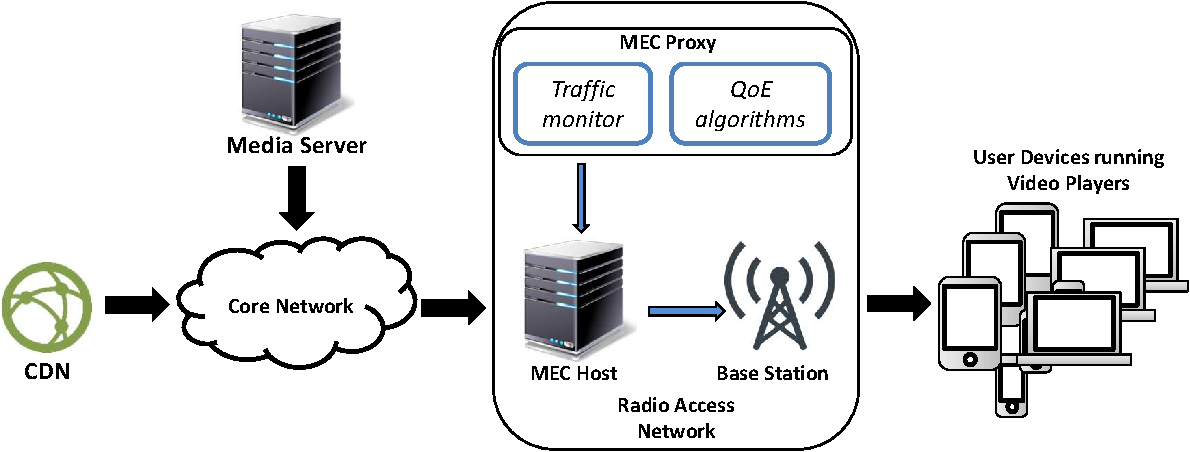
\includegraphics[width=1\textwidth]{architecture_updated.pdf}
	% figure caption is below the figure
	\caption{Architecture of MEC-based QoE estimation approach.}
	\label{fig:MTAP2020architecture} % Give a unique label
\end{figure}

To achieve it, the MEC Proxy is deployed at the MEC Host and monitors all the traffic exchanged at RAN between the video players, media server and CDN \cite{etsigsmec002}. During this operation, it can assess specific metrics related to the streaming session from two different activities:
\begin{itemize}
	\item download of video manifest from media server, which includes different metadata for each representation such as resolutions, nominal bitrates, or language for the different media streams;
	\item player's representation selection, when matching the HTTP segment requests with representations available in the manifest.
\end{itemize}

When a streaming session is started, the MEC Proxy downloads the video manifest and serves it to the player. The MEC Proxy can locally analyse the manifest to list the available representations and their features since the manifest includes information for all the available video, audio and subtitles tracks. Later, when the session is already playing, the video player must retrieve segments from the media server or CDN through HTTP requests. In this case, the MEC Proxy can act in two different ways:
\begin{enumerate}
	\item MEC Proxy can parse the information contained inside the HTTP URL and header as well as obtain request/response timestamps;
	\item MEC Proxy can analyse all the HTTP packets payload, meaning an active analysis of the media stream.
\end{enumerate}

Our solution is on top of first option to reduce the processing demands of the Proxy at the edge and favour a more scalable solution. In any case, it is security/privacy sensitive since standard encryption mechanisms of HAS standards just encrypts the payload of media segments to avoid unauthorized playback, so parsing the media manifest and process the HTTP requests endpoints are allowed.

The general communication is presented in Figure \ref{fig:MTAP2020communication}. First, the HTTP Proxy needs to identify each streaming session to link captured timestamps and QoE factors from each request and response to a specific item to infer its QoE metrics. To achieve it, the MEC Proxy generates a random ID when the first HTTP request from an IP requesting a manifest is received. Therefore, the MEC Proxy maintains a list with all the active streaming sessions. A session is considered expired when no HTTP requests are received during the duration of two segments. Then, inactive sessions are removed from the list.

\begin{figure}[htp]
	\centering
	% Use the relevant command to insert your figure file.
	% For example, with the graphicx package use
	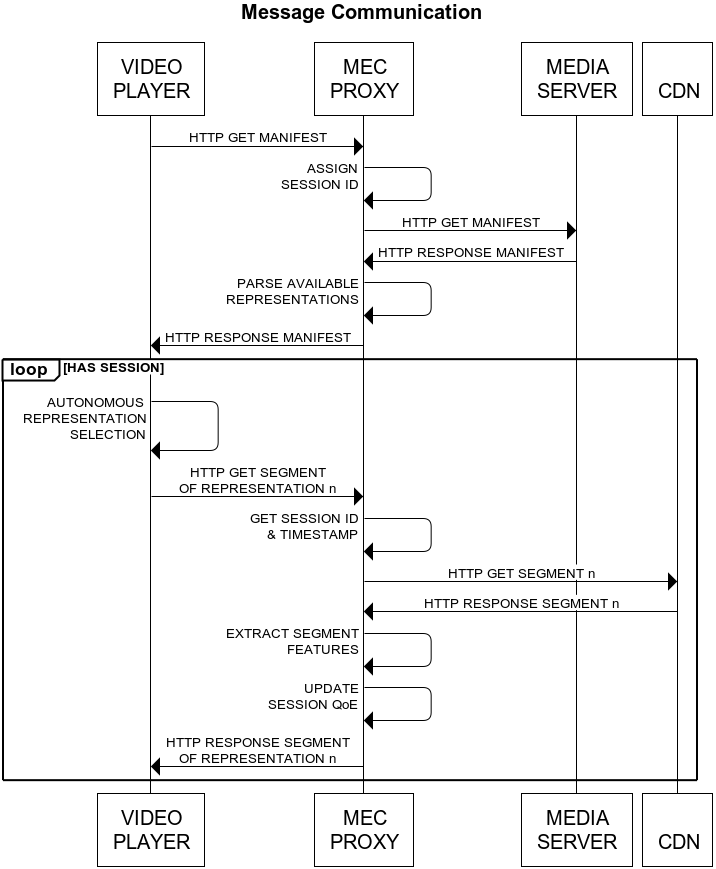
\includegraphics[width=0.8\textwidth]{comms.png}
	% figure caption is below the figure
	\caption{Message communication.}
	\label{fig:MTAP2020communication} % Give a unique label
\end{figure}

When the manifest is received by the video player it decides which representation better fits with the display features, the user preferences, the service subscription, and the network performance. This decision is revised by the video player for each segment to request. Accordingly, it starts to request a specific representation bitrate. The MEC Proxy stores the timestamps to later process request pace to detect any buffering issue when comparing nominal segment duration and time elapsed between requests. Then the MEC Proxy performs the CDN request and analyse some high-level features from the provided segment to accurately estimate the bitrate which may differ from the nominal value declared at the manifest. From that information, the MEC Proxy is can infer an estimated ITU-T P.1203 QoE. Last, the segment is delivered to the video player.

The list of sessions and the estimated QoE, updated for each segment request, is available for other systems at the edge or in the cloud to facilitate the enforcement or enhancement of video streaming in a dense client cell concerning QoE.


\subsubsection{QoE Estimation Algorithm}
\label{sec:MTAP202032}

ITU-T P.1203 \cite{itup1203} describes a model for monitoring media session quality while delivering content through HAS technologies. The building block of the ITU-T P.1203 model is presented in Figure \ref{fig:MTAP2020model}.

\begin{figure}[htp]
	\centering
	% Use the relevant command to insert your figure file.
	% For example, with the graphicx package use
	\includegraphics[width=1\textwidth]{p1203.png}
	% figure caption is below the figure
	\caption{Building blocks of the ITU-T P.1203 model. Source: \cite{itup1203}, Figure 1.}
	\label{fig:MTAP2020model} % Give a unique label
\end{figure}

The ITU-T P.1203 model receives media stream information and playback device features to generates the inputs (\textit{I.11, I.13, I.14, I.GEN}) for the internal modules (\textit{Pa, Pv, Pq, Pav, Pb}). The model generates the following input signals:

\begin{itemize}
	\item I.GEN: Playback display resolution and device type.
	\item I.11: Information on played audio segments, including audio codec and representation features.
	\item I.13: Information on played video segments, including video codec and representation features.
	\item I.14: Stalling event information, including stalling start time and its duration.
\end{itemize}

The inputs may be extracted or estimated in different ways since the ITU-T P.1203 does not provide information on \textit{Buffer parameter extraction} and \textit{Media parameter extraction} modules. The internal modules process the inputs signals to achieve several output QoE scores:
\begin{itemize}
	\item O.21 and O.22: \textit{Pa} and \textit{Pv} modules provide one score per sampling interval for audio and video, respectively.
	\item O.34, O.35 and O.23: \textit{Pav} and \textit{Pb} modules provides cumulative scores for audio-visual and buffering, respectively.
	\item O.46: \textit{Pq} module integrate audio-visual and buffering scores to provide the overall score.
\end{itemize}

All the outputs have 1-5 quality scale, where "1" means "bad" quality and "5" means "excellent" quality, according to MOS specifications \cite{Itu2016}.

The ITU-T P.1203 also establishes 4 modes of operation (mode 0 to 3) \cite{itup1203}. Mode 0 employs only content metadata. All the other modes work only with unencrypted content to acquire information from the media stream. Modes 2 and 3 also require decoding it. Consequently, if we employ mode 1-3 at the MEC Proxy, it may cause security issues. For this reason, we employ mode 0 for our MEC Proxy. Moreover, mode 0 is also the less intensive in terms of processing.

A software implementation of ITU-T P.1203 standard internal modules is provided in \cite{itugithub}. The software implements the internal modules \cite{Robitza2018} according to the ITU-T P.1203 and provides customized \textit{Media parameter extraction} and \textit{Buffer parameter extraction} modules (the ITU-T P.1203 does not specifies these modules). These customized modules are useful to generate compliant inputs signals and evaluate the internal modules, but they are limited for working with locally stored video files. So, they could not be used while streaming a content. All the modules provided by this software implementation are also capable to analyse the media content through any of the four available modes \cite{raake2017}.

To feed the ITU-T P.1203 while streaming a content, we have designed and implemented our custom solutions to generate the inputs. \textit{I.GEN} can be easily known by analysing the header of the HTTP requests since it contains a User-Agent field \cite{useragent} that allows the recognition of the HTTP client type (mobile or desktop device, browser or application, etc.), while keeping anonymous the identity of the user. To extract the remain input signals, we design both \textit{Media parameter extraction} and \textit{Buffer parameter extraction} modules which execute Algorithm \ref{alg:algorithmMedia} and Algorithm \ref{alg:algorithmBuffer}, respectively.

\begin{algorithm}
	\renewcommand{\algorithmicrequire}{\textbf{Input:}}
	\renewcommand{\algorithmicensure}{\textbf{Output:}}
	\caption{Media parameter extraction}
	\label{alg:algorithmMedia}
	\begin{algorithmic}
		\Function{mediaParameter}{Manifest, segment$_n$, \{segment\}$_{n-1}$} \Comment{for each downloaded segment}
		%\parbox[t]{.5\linewidth}{} \linebreak
		\Require Manifest \Comment{media manifest}
		\Require segment$_n$ \Comment{current downloaded segment}
		\Require \{segment\}$_{n-1}$ \Comment{session information including last segment}
		\Ensure \{segment\}$_{n}$ \Comment{session information updated with current segment}
		\State d$_n$, res$_n$, fps$_n$, codec$_n$ $\leftarrow$ parseManifest(Manifest, segment$_n$) \Comment{segment duration, resolution, framerate and codec}
		\State size$_n$ $\leftarrow$ getBitSize(segment$_n$) \Comment{current segment size}
		\State bitrate$_n$ = $\frac{size_n}{d_n}$ \Comment{current segment bitrate}
		\State \{segment$_n$\} = \{d$_n$, res$_n$, fps$_n$, codec$_n$, bitrate$_n$\} \Comment{current segment information}
		\State \{segment\}$_n$ $\leftarrow$ \{\{segment\}$_{n-1}$, \{segment$_n$\}\} \Comment{updated session information}
		\EndFunction
	\end{algorithmic}
\end{algorithm}

The Algorithm \ref{alg:algorithmMedia} is executed for each segment downloaded by the MEC Proxy. It receives the media manifest, the most recent downloaded segment, and the accumulated metadata for the past downloaded segments of a specific session. In the case of employing MPEG-DASH video streaming technology, the manifest would be a Media Presentation Description (MPD). First, specific metadata is captured by matching the manifest and the segment URL, identifying the specific selected representation by the video player for each segment time slot. Second, a more accurate metric in terms of the actual bitrate is captured from the segment size and its nominal duration. Usually, the duration of the segments is fixed as the Group of Pictures (GOP) size is fixed at the encoders to start the segment with a keyframe, so the nominal duration declared in the manifest is accurate. Once all the metadata for the current segment (\{segment$_n$\}) are collected, i.e., bitrate, duration, resolution, framerate and employed codec, this information is stored for all the session long (\{segment\}$_n$), updating the series for the last downloaded segment (\{segment\}$_{n-1}$).

\begin{algorithm}
	\renewcommand{\algorithmicrequire}{\textbf{Input:}}
	\renewcommand{\algorithmicensure}{\textbf{Output:}}
	% \caption{Stall Estimation}
	\caption{Buffer parameter extraction}
	\label{alg:algorithmBuffer}
	\begin{algorithmic}
		% \Function{stallEstimation}{n, d, t$_0$, t$_n$, \{stall\}$_{n-1}$} \Comment{for each downloaded segment}
		\Function{bufferParameter}{n, d, t$_0$, t$_n$, \{stall\}$_{n-1}$} \Comment{for each downloaded segment}
		\Require n \Comment{segment index}
		\Require d \Comment{segment duration}
		\Require t$_0$ \Comment{first segment download time}
		\Require t$_n$ \Comment{current segment download time}
		\Require \{stall\}$_{n-1}$ = \{\{start$^{stall}_0$, d$^{stall}_0$\},...,\{start$^{stall}_k$, d$^{stall}_k$\}\} \Comment{session stalls including last segment}
		\Ensure \{stall\}$_n$ \Comment{session stalls updated with current segment}
		\State $k$ $\leftarrow$ \{stall\}$_{n-1}$ \Comment{number of estimated stalls along the session}
		\State D$^{stall}$ = $\sum_{i=0}^{k}$ d$^{stall}_i$ \Comment{total duration of estimated stalls along the session}
		\State t$_{playback}$ = (t$_n$ - t$_0$) - D$^{stall}$ \Comment{playback time}
		\State d$_{downloaded}$ = (n-1)*d \Comment{total duration of downloaded segments}
		\State d$^{stall}$ = t$_{playback}$ - d$_{downloaded}$ \Comment{candidate stall duration}
		\If {(d$^{stall}$ $>$ 0)} \Comment{check if stalling in the recent segment}
		\State d$_{k+1}^{stall}$ = d$^{stall}$ \Comment{record stall duration}
		\State start$_{k+1}^{stall}$ = t$_n$ - d$^{stall}$ \Comment{stall start time}
		\State \{stall$_{k+1}$\} = \{start$_{k+1}^{stall}$, d$_{k+1}^{stall}$\} \Comment{estimated parameters of new stall (start time and duration)}
		\State \{stall\}$_n$ = \{\{stall\}$_{n-1}$, \{stall$_{k+1}$\}\} \Comment{update stall series}
		\State $k$++ \Comment{new stall when playing the current segment}
		\Else
		\State \{stall\}$_n$ = \{stall\}$_{n-1}$ \Comment{unchanged stall information}
		\EndIf
		\EndFunction
	\end{algorithmic}
\end{algorithm}

The Algorithm \ref{alg:algorithmBuffer} is executed at the MEC Proxy once each segment download is completed by the video player. It estimates stall occurrence and duration without access to video player buffer or playback issues. The MEC Proxy is remotely inferring the playback issues from the timestamps on video player requests. As the video players download a new segment once another has been played, the inter-arrival on video player requests should follow segment duration. Any identified drift likely means a buffering issue. To this end, this function, also executed for each downloaded segment, gets the duration of the segment, the download timestamps of the video player from the segment provided by the MEC Proxy, and the records of past estimations of stalls for previous segment time slots in the session. First, the total duration of estimated stalls along the session is calculated.
Then, the current playback time is measured from the elapsed time from the player's start-up to the last downloaded segment, including the total estimated stall for all the session. The MEC Proxy assumes the first downloaded segment time as the start-up time. It is a reasonable choice since the player starts decoding and displaying the content only when the first segment is completely downloaded. With this assumption, an error could be introduced on the start-up time selection since the proxy cannot measure decoding delay of the first frame. In any case, decoding operation is done in real time, meaning that the maximum error is in the order of tens of milliseconds (1/framerate). Downloading time duration and player's internal buffer size are in the same order of magnitude of segment duration (seconds), which is 100 times higher than the decoding delay. Thus, the error due to decoding delay has a negligible impact on the overall measurement of the start-up time.
To calculate the duration of content available at the video player, the algorithm only includes the previously downloaded segments ($n-1$) excluding the most recent one ($n$). As this function is evaluated just once the segment has been downloaded by the video player, the most recent segment has not been decoded yet. If the current playback time (t$_{playback}$) is lower than the duration of content available at the video player (d$_{downloaded}$), the video player has buffered content to be played, so stall should not happen. If the playback time is ahead the duration of available content, the stall duration is estimated (d$^{stall}$), and the start time of this stall is assumed shifting current segment download time (t$_n$). Last, estimated timestamp and duration of detected stall is stored.

\subsection{Results}

\label{sec:MTAP20204}
\subsubsection{Experimental setup}
\label{sec:MTAP202041}

To demonstrate the effectiveness of the proposed approach to assess the ITU-T P.1203 \cite{itup1203} QoE scores, we deployed the testbed shown in Figure \ref{fig:MTAP2020testbed}. The experimental setup comprises the following:
\begin{itemize}
	\item Media server: we use a mirror server located at Polytechnic University of Turin and belonging to D-DASH dataset and infrastructure \cite{lederer2013} which provides a Dynamic Adaptive Streaming over HTTP (DASH) standard content.
	\item MEC proxy and access point: this is a unique node deployed through a Node.js \cite{nodejs} proxy application running on a Raspberry Pi 3 single-board computer \cite{richardson2012}. Raspberry Pi 3 includes both computing capabilities to execute edge processing and a WiFi internal module to deploy a local wireless network such to provide connection to WiFi clients. Thus, this design guarantees ultra-low latency, proximity and high bandwidth \cite{etsigsmecwifi}. This node has Internet access to download the MPD and the corresponding media segments stored at the Media Server which are served to the clients on demand.
	\item UE node: client node featuring WiFi interface and running several DASH players, based on GStreamer multimedia framework \cite{gstreamer}, which download the video stream. Players run headless (without GUI) since we are not interested in displaying the content and allowing the client to save computing capabilities.
\end{itemize}

% For two-column wide figures use
\begin{figure}[htp]
	\centering
	% Use the relevant command to insert your figure file.
	% For example, with the graphicx package use
	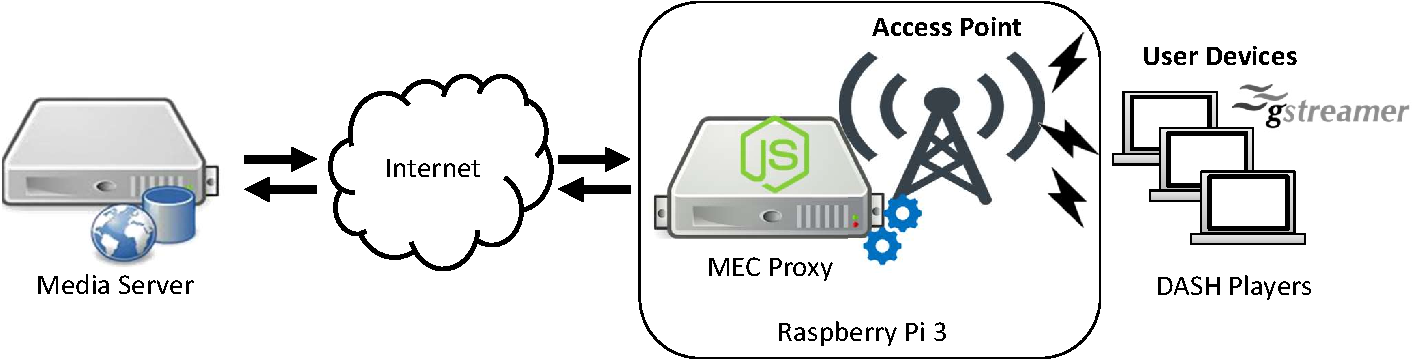
\includegraphics[width=1\textwidth]{testbed_updated.pdf}
	% figure caption is below the figure
	\caption{Testbed.}
	\label{fig:MTAP2020testbed} % Give a unique label
\end{figure}
%

Node.js application at MEC node employs \textit{http-server} module for acquiring HTTP request and response time and \textit{xml2js} module for parsing the MPD to feed Algorithms 1 and 2. During the experiments, Algorithms 1 and 2 are also implemented inside Node.js application and run in real time to generate the inputs of ITU-T P.1203 model. However, ITU-T P.1203 QoE evaluation is performed offline, after that all the metrics are collected. Thus, it simplifies the process of metrics collection and QoE evaluation, while the QoE results remain valid as the input metrics for the ITU-T P.1203 model do not change.

The dataset at the Media Server includes the Red Bull Playstreet video sequence, which is owned by Red Bull Media House and licensed for scientific purposes. This sequence is encoded for 17 video representations through advanced video coding (H.264/AVC) and 4 dual channel audio representations through advanced audio coding (AAC). Both audio and video are segmented with different segment lengths of 2, 4, 6, 10, and 15 seconds, and multiplexed in ISO MPEG4 files (ISO/IEC \hbox{14496-12} - \hbox{MPEG-4} Part 12). For our experiments, we employed 6 seconds segments as such duration favour accuracy of the proposed solution when delivering segments with enough size in bytes to get a more solid assessment of the network performance while downloading, while the serving latency is still valid for streaming of live events.

The representations range from a resolution of 320 x 240 and 30 fps at 100 kbps to a resolution of 1920 x 1080 and 30 fps at 6000 kbps. As the client-side bitrate adaptation mechanism does not target a specific resolution, then each client struggles to achieve the highest representation bitrate.

We use the outcomes of \cite{yu2006} to model players behaviour. The authors provide an extensive analysis on user behaviour while accessing streaming services. The player inter-arrival time fits a modified version of the Poisson distribution. This means that the players are starting and stopping their sessions (joining and leaving the cell/hotspot) along the experiment according to a Poisson distributed inter-arrival time. Moreover, the duration of streaming sessions of the players is variable and follows the declared sections of 5 (37.44\%), 10 (52.55\%), or 25 min (75.25\%). As a result, the effective number of players employed during the experiments is variable since the model is aleatory. Modelling players inter-arrival time and their streaming session duration according to a real distribution allows to emulate a real media traffic scenario.

To test with different network loads, we also consider two different scenarios where we change the limit of the maximum number of concurrent players:

\begin{itemize}
	\item Scenario 1: 10 players at a time. Here, no more than 10 players at a time are connected to the WiFi access node and downloading the content.
	\item Scenario 2: 20 players at a time. The number of players concurrently consuming the video streaming is increased to 20.
\end{itemize}

We perform a test over each scenario for one hour. It results in 66 players taking part in the first scenario and 144 players participating in the second scenario.


%%%%%%%%%%%%%%%%%%%%%%%%%%%%%%%%%%%%%%%%%%%%%%%%%%%%%%%%%%%%%%%%%%%%%%%%%
\subsubsection{Evaluation metrics}
\label{sec:MTAP202042}

To evaluate the proposed solution, we employ the outputs of the ITU-T P.1203, which provide subjective evaluation of the streaming sessions. Since we are focused on evaluating QoE of video representation, we target the following outputs from the ones analysed by ITU-T P.1203:

\begin{itemize}
	\item O.34: it provides a video quality score per output sampling interval. The default interval of the ITU-T P.1203 implementation is 1s, so we have 6 new values per every downloaded segment.
	\item O.23: it provides overall score considering stalling events. We update this value every time the player downloads a new segment.
	\item O.46: it provides overall score overall quality score, considering video and stalling events. We update this value every time the player downloads a new segment.
\end{itemize}

To check the accuracy of the values obtained by the MEC Proxy, we compare the outcomes at the MEC with the outputs at the player side. At the player it is not necessary to design algorithms to extract, estimate or infer the target signals of the ITU-T P.1203 model since all of them are directly available at the video player. The player establishes the video representation, then it knows the features of the downloaded segment after selecting one. Moreover, to know if a stall is experienced, it is enough to check when the internal playback buffer goes empty.

\subsubsection{QoE estimation at the Edge results}
\label{sec:MTAP202043}

\begin{figure}[htp]
	\centering
	\subfloat[]{
		% Use the relevant command to insert your figure file.
		% For example, with the graphicx package use
		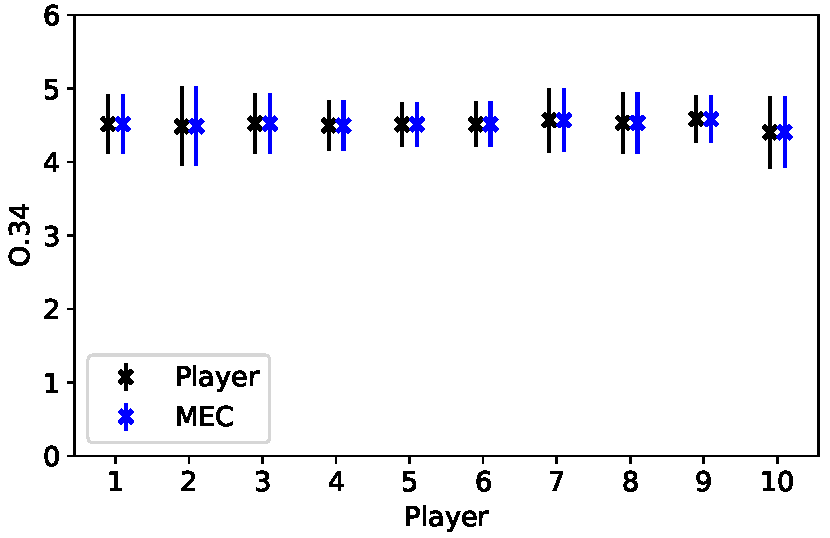
\includegraphics[width=0.6\textwidth]{O34.pdf}
		% figure caption is below the figure
		\label{fig:MTAP2020O34}
	}
	\hfil
	\subfloat[]{
		% Use the relevant command to insert your figure file.
		% For example, with the graphicx package use
		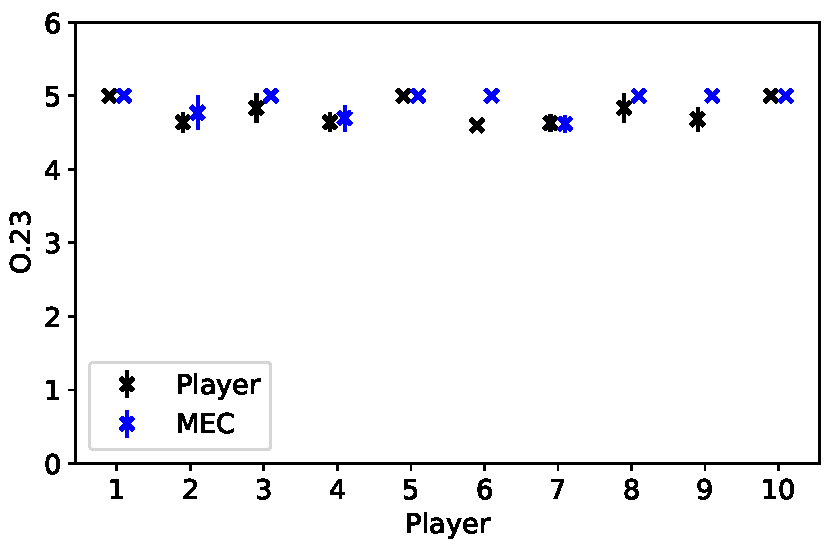
\includegraphics[width=0.6\textwidth]{O23.pdf}
		% figure caption is below the figure
		\label{fig:MTAP2020O23}
	}
	\hfil
	\subfloat[]{
		% Use the relevant command to insert your figure file.
		% For example, with the graphicx package use
		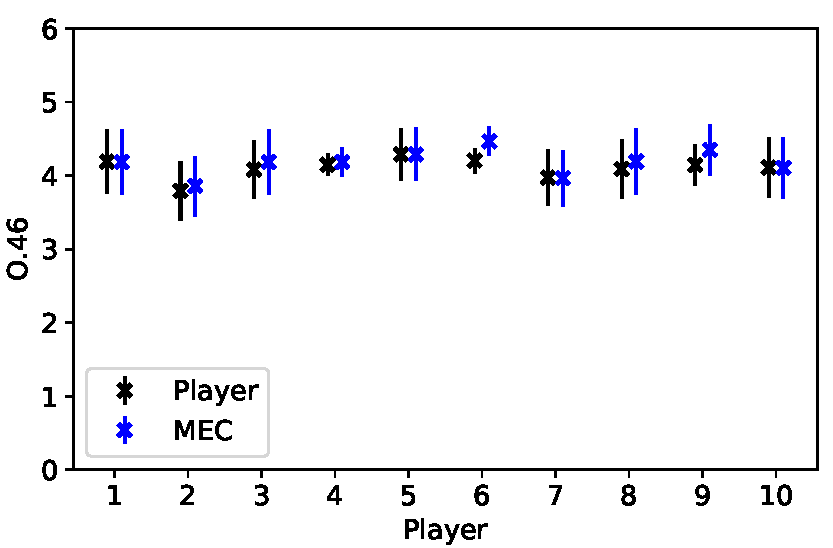
\includegraphics[width=0.6\textwidth]{mos.pdf}
		% figure caption is below the figure
		\label{fig:MTAP2020O46}
	}
	\hfil
	\caption{Average and standard deviation of ITU-T P.1203 QoE scores for 10 players from Scenario 2: O.34 (a), O.23 (b) and O.46 (c).}
	\label{fig:MTAP2020mos} % Give a unique label
\end{figure}

As described in Section \ref{sec:MTAP202041}, the player inter-arrival time and session duration are modelled as described at \cite{yu2006}. While testing the proposed solution for one hour, it resulted in 66 video players for Scenario 1 and 144 for Scenario 2. In terms of computational capabilities consumption, Raspberry Pi 3, which runs the MEC Proxy (Algorithms 1 and 2) and the access point, experiences 13\% CPU and 122MB RAM usage during Scenario 1 and 17\% CPU and 156MB RAM usage during Scenario 2.

\begin{table}[htp]
	\caption{Scenario 1: number (N$_{stall}$) and total duration (T$_{stall}$) of stalls.}
	\centering
	\bgroup
	\def\arraystretch{1.2}%  1 is the default, change whatever you need
	\setlength\tabcolsep{2.5pt} % default value: 6pt
	\label{tab:MTAP2020stall1}
	{\scriptsize
		\begin{tabular}{>{\centering\arraybackslash}m{\dimexpr0.1\textwidth-2\tabcolsep-\arrayrulewidth\relax}
				>{\centering\arraybackslash}m{\dimexpr0.1\textwidth-2\tabcolsep-\arrayrulewidth\relax}
				>{\centering\arraybackslash}m{\dimexpr0.1\textwidth-2\tabcolsep-\arrayrulewidth\relax}
			}
			\toprule
			& \textbf{N$_{\textbf{stall}}$} & \textbf{T$_{\textbf{stall}}$} \\
			\midrule
			\midrule
			\textbf{Player} & 661 & 289s \\
			\textbf{MEC} & 160 & 263s \\
			\bottomrule
			\bottomrule
		\end{tabular}
	}
	\egroup
\end{table}

\begin{table}[htp]
	\caption{Scenario 2: number (N$_{stall}$) and total duration (T$_{stall}$) of stalls.}
	\centering
	\bgroup
	\def\arraystretch{1.2}%  1 is the default, change whatever you need
	\setlength\tabcolsep{2.5pt} % default value: 6pt
	\label{tab:MTAP2020stall2}
	{\scriptsize
		\begin{tabular}{>{\centering\arraybackslash}m{\dimexpr0.1\textwidth-2\tabcolsep-\arrayrulewidth\relax}
				>{\centering\arraybackslash}m{\dimexpr0.1\textwidth-2\tabcolsep-\arrayrulewidth\relax}
				>{\centering\arraybackslash}m{\dimexpr0.1\textwidth-2\tabcolsep-\arrayrulewidth\relax}
			}
			\toprule
			& \textbf{N$_{\textbf{stall}}$} & \textbf{T$_{\textbf{stall}}$} \\
			\midrule
			\midrule
			\textbf{Player} & 1623 & 757s \\
			\textbf{MEC} & 334 & 765s \\
			\bottomrule
			\bottomrule
		\end{tabular}
	}
	\egroup
\end{table}

Figure \ref{fig:MTAP2020mos} shows average value and standard deviation along the streaming session of the considered ITU-T P.1203 outputs. It shows only the results for 10 players randomly chosen among the executed ones of the Scenario 2 since it is the most demanding scenario, where more stalls and quality changes are experienced. Scenario 1 has similar results, but as expected the average values are higher due to the lower competition for the available network resources. The results for O.34 (Figure \ref{fig:MTAP2020O34}) obtained at the MEC are like the ones obtained at the player. It is reasonable since most of the video information to provide to the ITU-T P.1203 model comes from the MPD, which is available at the player, as well as at the MEC Proxy. On the contrary, the results for O.23 (Figure \ref{fig:MTAP2020O23}) shows some differences since the Algorithm \ref{alg:algorithmBuffer} may not detect all the stalling events at the player side from the MEC Proxy. The sampling time to check for stalls at the MEC Proxy is equal to the segment duration. Then, a stall experienced by the player, whose duration is short, and it is recovered before the next check at the MEC, may not be detected correctly. Consequently, estimated values at the MEC are higher that the captured ones at the player. Tables \ref{tab:MTAP2020stall1} and \ref{tab:MTAP2020stall2} also provides more in-depth details of the stalls. It is clear from the tables that the MEC cannot detect all the stalls. Anyway, the total duration of stalls tends to actual one experienced by the player. It means that MEC Proxy cannot detect micro-stalls and tends to concentrate several of them into a macro-stall. Again, this is due to the sampling time to check for stalls. If two micro-stalls are experienced during the same segment, the MEC Proxy will consider that they are one longer stall since it checks only at the end of each segment download. Finally, O.46 scores (Figure \ref{fig:MTAP2020O46}) are directly influenced by the results obtained by the other two scores (O.34 and O.23). It has a significant standard deviation due to video scores (O.34), but lower average value due to the impact of buffering score (O.23).

Tables \ref{tab:MTAP2020results11} and \ref{tab:MTAP2020results12} resume the scores of all the players executed under the Scenarios 1 and 2, respectively. The Tables shows the results by averaging the values obtained by the players and evaluating the standard deviation for each considered score. The Tables confirms that O.34 has the same values when estimated at the MEC and captured at the player, while O.23 scores assessed at the MEC tends to be higher than the real values issued at the player. Again, O.46 scores, which are influenced by the other two scores, shows a standard deviation coming from O.34 and lower average values inherited from O.23.

\begin{table}[htp]
	\caption{Scenario 1: average and standard deviation of ITU-T P.1203 QoE scores.}
	\centering
	\bgroup
	\def\arraystretch{1.2}%  1 is the default, change whatever you need
	\setlength\tabcolsep{2.5pt} % default value: 6pt
	\label{tab:MTAP2020results11}
	{\scriptsize
	\begin{tabular}{>{\centering\arraybackslash}m{\dimexpr0.1\textwidth-2\tabcolsep-\arrayrulewidth\relax}
			>{\centering\arraybackslash}m{\dimexpr0.1\textwidth-2\tabcolsep-\arrayrulewidth\relax}
			>{\centering\arraybackslash}m{\dimexpr0.1\textwidth-2\tabcolsep-\arrayrulewidth\relax}
			>{\centering\arraybackslash}m{\dimexpr0.1\textwidth-2\tabcolsep-\arrayrulewidth\relax}
			>{\centering\arraybackslash}m{\dimexpr0.1\textwidth-2\tabcolsep-\arrayrulewidth\relax}
			>{\centering\arraybackslash}m{\dimexpr0.1\textwidth-2\tabcolsep-\arrayrulewidth\relax}
			>{\centering\arraybackslash}m{\dimexpr0.1\textwidth-2\tabcolsep-\arrayrulewidth\relax}
		}
		\toprule
		& \textbf{O.34$_{\textbf{avg}}$} & \textbf{O.34$_{\textbf{std}}$} & \textbf{O.23$_{\textbf{avg}}$} & \textbf{O.23$_{\textbf{std}}$} & \textbf{O.46$_{\textbf{avg}}$} & \textbf{O.46$_{\textbf{std}}$} \\
		\midrule
		\midrule
		\textbf{Player} & 4.71 & 0.28 & 4.81 & 0.20 & 4.38 & 0.28 \\
		\textbf{MEC} & 4.70 & 0.28 & 4.84 & 0.19 & 4.39 & 0.28 \\
		\bottomrule
		\bottomrule
	\end{tabular}
	}
	\egroup
\end{table}

\begin{table}[htp]
	\caption{Scenario 2: average and standard deviation of ITU-T P.1203 QoE scores.}
	\centering
	\bgroup
	\def\arraystretch{1.2}%  1 is the default, change whatever you need
	\setlength\tabcolsep{2.5pt} % default value: 6pt
	\label{tab:MTAP2020results12}
	{\scriptsize
	\begin{tabular}{>{\centering\arraybackslash}m{\dimexpr0.1\textwidth-2\tabcolsep-\arrayrulewidth\relax}
			>{\centering\arraybackslash}m{\dimexpr0.1\textwidth-2\tabcolsep-\arrayrulewidth\relax}
			>{\centering\arraybackslash}m{\dimexpr0.1\textwidth-2\tabcolsep-\arrayrulewidth\relax}
			>{\centering\arraybackslash}m{\dimexpr0.1\textwidth-2\tabcolsep-\arrayrulewidth\relax}
			>{\centering\arraybackslash}m{\dimexpr0.1\textwidth-2\tabcolsep-\arrayrulewidth\relax}
			>{\centering\arraybackslash}m{\dimexpr0.1\textwidth-2\tabcolsep-\arrayrulewidth\relax}
			>{\centering\arraybackslash}m{\dimexpr0.1\textwidth-2\tabcolsep-\arrayrulewidth\relax}
		}
		\toprule
		& \textbf{O.34$_{\textbf{avg}}$} & \textbf{O.34$_{\textbf{std}}$} & \textbf{O.23$_{\textbf{avg}}$} & \textbf{O.23$_{\textbf{std}}$} & \textbf{O.46$_{\textbf{avg}}$} & \textbf{O.46$_{\textbf{std}}$} \\
		\midrule
		\midrule
		\textbf{Player} & 4.53 & 0.31 & 4.76 & 0.19 & 4.22 & 0.27 \\
		\textbf{MEC} & 4.53 & 0.31 & 4.85 & 0.20 & 4.28 & 0.28 \\
		\bottomrule
		\bottomrule
	\end{tabular}
	}
	\egroup
\end{table}

As expected, Scenario 1 presents higher values for any of the considered metrics since the network resources are the same as Scenario 2, but the number of players sharing them is lower. The resulting standard deviations are similar for both scenarios.

Tables \ref{tab:MTAP2020results21} and \ref{tab:MTAP2020results22} compare the results obtained at the MEC and at the player side by providing the Mean Absolute Error (MAE) and Root Mean Square Error (RMSE) between the different scores. The results show that the scores obtained at the MEC tends to be like the ones obtained at the player, achieving more accurate results in the Scenario 1, as expected.

\begin{table}[htp]
	\caption{Scenario 1: MAE and RMSE for ITU-T P.1203 QoE scores.}
	\centering
	\bgroup
	\def\arraystretch{1.2}%  1 is the default, change whatever you need
	\setlength\tabcolsep{2.5pt} % default value: 6pt
	\label{tab:MTAP2020results21}
	{\scriptsize
	\begin{tabular}{>{\centering\arraybackslash}m{\dimexpr0.1\textwidth-2\tabcolsep-\arrayrulewidth\relax}
			>{\centering\arraybackslash}m{\dimexpr0.1\textwidth-2\tabcolsep-\arrayrulewidth\relax}
			>{\centering\arraybackslash}m{\dimexpr0.1\textwidth-2\tabcolsep-\arrayrulewidth\relax}
			>{\centering\arraybackslash}m{\dimexpr0.1\textwidth-2\tabcolsep-\arrayrulewidth\relax}
		}
		\toprule
		& \textbf{O.34} & \textbf{O.23} & \textbf{O.46} \\
		\midrule
		\midrule
		\textbf{MAE} & 0.21 & 0.11 & 0.18 \\
		\textbf{RMSE} & 0.39 & 0.21 & 0.36 \\
		\bottomrule
		\bottomrule
	\end{tabular}
	}
	\egroup
\end{table}

\begin{table}[htp]
	\caption{Scenario 2: MAE and RMSE for ITU-T P.1203 QoE scores.}
	\centering
	\bgroup
	\def\arraystretch{1.2}%  1 is the default, change whatever you need
	\setlength\tabcolsep{2.5pt} % default value: 6pt
	\label{tab:MTAP2020results22}
	{\scriptsize
	\begin{tabular}{>{\centering\arraybackslash}m{\dimexpr0.1\textwidth-2\tabcolsep-\arrayrulewidth\relax}
			>{\centering\arraybackslash}m{\dimexpr0.1\textwidth-2\tabcolsep-\arrayrulewidth\relax}
			>{\centering\arraybackslash}m{\dimexpr0.1\textwidth-2\tabcolsep-\arrayrulewidth\relax}
			>{\centering\arraybackslash}m{\dimexpr0.1\textwidth-2\tabcolsep-\arrayrulewidth\relax}
		}
		\toprule
		& \textbf{O.34} & \textbf{O.23} & \textbf{O.46} \\
		\midrule
		\midrule
		\textbf{MAE} & 0.14 & 0.14 & 0.19 \\
		\textbf{RMSE} & 0.43 & 0.24 & 0.36 \\
		\bottomrule
		\bottomrule
	\end{tabular}
	}
	\egroup
\end{table}

Note that O.34 has higher MAE and RMSE than O.23 and O.46. It could be considered a contradictory to the fact that the values obtained at MEC Proxy compared to the values captured at the player for O.34 are more accurate than O.23 and O.46. Anyway, it is important to remember that these metrics have different sampling rates. O.34 provides a value every second, while O.23 and O.46 every segment (6s). Then, O.34 has higher values for MAE and RMSE since they are evaluated over a number of scores which is 6 times bigger than O.23 and O.46. Finally, if we compare the two scenarios, the results tend to be similar since the MAE and RMSE are relative values, they are not conditioned by the average values of the metrics. It means that the MEC Proxy performs similarly in both scenarios.

In summary, the proposed MEC Proxy can monitor network dynamics and estimate the individual QoE of each player according to Recommendation ITU-T P.1203. The results show that video related scores (O.34) estimated follow the actual ones captured at the player, while buffering scores (O.23) tend to miss some small stalls unperceived from segment to segment. Anyway, the overall scores (O.46) are still valid showing a small difference of the estimated values at the MEC from the actual values captured at the player.

\subsection{Conclusion}
\label{sec:MTAP20205}

The trend for the following years is an increasing consumption of media content due to the popularity of video streaming platforms. To cope with this increasing demand, MNOs need to manage the network according to cost-effective policies, requiring monitoring solutions which provide actionable data to management systems to provide the best QoE with the available network resources.

The proposed 5G MEC-enabled proxy aims to estimate the ITU-T P.1203 QoE metrics to enable edge services operating coordinated decisions on the streaming qualities. The MEC Proxy assesses QoS metrics at the radio cell and parses manifests of requested DASH streams to estimate the parameters employed to evaluate ITU-T P.1203 QoE scores. Consequently, there is no need for explicit out-of-band messaging from video players to send playback statistics to the MEC.

The solution has been implemented in a real testbed where WiFi was employed as access network between MEC and players and tested in two scenarios with different demands and traffic loads over the network. The results demonstrate the capability of the MEC Proxy to estimate ITU-T P.1203 QoE scores close to actual ones.

\subsection*{Acknowledgment}
This work was fully supported by the 5G-TEST project (Gipuzkoa's research and innovation programme) and Open-VERSO project (Red Cervera program, Spanish government's Centre for the Development of Industrial Technology).
		
